\chapter{Physical Elements and Markers}
\label{sec:element}
\index{element|(}
\index{physical!element}

\section{Element Input Format}
\label{sec:elm-format}
\index{element!format}
\index{format!element}
All physical elements are defined by statements of the form
\begin{verbatim}
label:keyword,attribute,...,attribute
\end{verbatim}
\noindent Example:
\begin{verbatim}
QF: QUADRUPOLE,L=1.8,K1=0.015832;
\end{verbatim}
where
\begin{description}
\item[label]
  \index{element!label}
  \index{label!element}
  Is the name to be given to the element (in the example QF),
  it is an \secref{\texttt{identifier}}{label}.
\item[keyword]
  \index{element!keyword}
  \index{keyword!element}
  Is a \secref{\texttt{keyword}}{label},
  it is an element type keyword (in the example \texttt{QUADRUPOLE}),
\item[attribute]
  \index{element!attribute}
  \index{attribute!element}
  normally has the form
\begin{verbatim}
attribute-name=attribute-value
\end{verbatim}
\item[attribute-name]
  \index{attribute!name}
  \index{name!attribute}
  selects the attribute from the list defined for the element type 
  \texttt{keyword} (in the example \texttt{L} and \texttt{K1}).
  It must be an \secref{\texttt{identifier}}{label} 
\item[attribute-value]
  \index{attribute!valu}
  \index{value!attribute}
  gives it a \secref{\texttt{value}}{attribute} 
  (in the example \texttt{1.8} and \texttt{0.015832}).
\end{description}
Omitted attributes are assigned a default value, normally zero.


\section{Element Classes}
\label{sec:elm-class}
\index{element!class}
\index{class!of elements}
The concept of element classes solves the problem of addressing
instances of elements in the accelerator in a convenient manner.
It also helps defining portions of the machine which are shared
physically between two or more beam lines.

This concept will first be illustrated by an example.
All the quadrupoles in the accelerator form a class \texttt{QUADRUPOLE}.
Let us define three subclasses for the focussing quadrupoles,
the defocussing quadrupoles, and the skewed quadrupoles:
\begin{verbatim}
MQF:QUADRUPOLE,L=LQM,K1=KQD; // Focusing quadrupoles
MQD:QUADRUPOLE,L=LQM,K1=KQF; // Defocusing quadrupoles
MQT:QUADRUPOLE,L=LQT;        // Skewed quadrupoles
\end{verbatim}
These classes can be thought of as new keywords which define elements
with specified default attributes. 
We now use them to define the real quadrupoles:
\begin{verbatim}
QD1:MQD; // Defocusing quadrupoles
QD2:MQD;
QD3:MQD;
...
QF1:MQF; // Focusing quadrupoles
QF2:MQF;
QF3:MQF;
...
QT1:MQT,K1S=KQT1; // Skewed quadrupoles
QT2:MQT,K1S=KQT2;
...
\end{verbatim}
These quadrupoles inherit all unspecified attributes from their class.
This allows to build up a hierarchy of objects with a rather
economic input structure.

The full power of the class concept is revealed when object classes
are used to \secref{select}{select} instances of elements for printing.
\noindent Example:
\begin{verbatim}
SELECT,CLASS=QUADRUPOLE;  // Select all quadrupoles
PRINT,CLASS=MQT;          // Select skewed quadrupoles
\end{verbatim}

More formally, for each element keyword \opal maintains a class of
elements with the same name. 
A defined element becomes itself a class which can be used to define
new objects, 
which will become members of this class.
A new object inherits all attributes from its class;
but its definition may override some of those values by new ones.
All class and object names can be used in range selections,
providing a powerful mechanism to specify positions
for matching constraints and printing.

When an object is used in a beam line,
\opal automatically makes a copy of that element,
unless the object is defined as \texttt{SHARED}.
The user can later attach imperfections to all copies individually.
Example:
\begin{verbatim}
QF:QUADRUPOLE,...;          // Define the class QF
L:LINE=(...,QF,...,QF,...)  // Each QF is distinct
QF1:QF,...;                 // QF1 is derived from QF
\end{verbatim}

On the contrary, if an object is defined as shared using the keyword
\texttt{SHARED}, 
\index{shared element}
\index{element!shared}
\index{SHARED}
its use in more than one beam line implies the same object occurs
in all those beam lines.
Example:
\begin{verbatim}
SHARED QF:QUADRUPOLE,...;   // Define shared quadrupole QF
L1:LINE=(...,QF,...,QF,...) // All the QF's are the same ...
L2:LINE=(...,QF,...)        // ... also in this line.
\end{verbatim}
This is a restricted feature: \noopalt, \noopalcycl.

\section{Common Attributes for all Elements}
\label{sec:common}
The following attributes are allowed on all elements:
\begin{description}
\item[TYPE]
  \index{TYPE}
  A \secref{\texttt{string value}}{astring}.
  It specifies an ``engineering type'' and can be used for element
  selection.
\item[APERTURE]
  \index{APERTURE}
  A real vector with an arbitrary length which describes
  the element aperture.
  It is ignored by \opal, but it can be used in other programs.
\item[WAKEF]
  \index{WAKEF}
Defines the type of wake to be applied: \texttt{WT,WL} or \texttt{WTL} for 
transverse, longitudinal or both.
\item[other]
  \index{unknown attribute}
  \index{attribute!unknown}
  All elements can have arbitrary additional attributes
  which are not defined below.
  Such attributes must have a name different from all defined attributes
  and single real values.
\end{description}
Only the \texttt{TYPE} attribute is used by \opal,
but the \secref{\texttt{SAVE} command}{save} saves all attributes.

\section{Thin Lenses}
\label{sec:thin}
\index{thin lens}
All multipole-like elements
(\texttt{RBEND, SBEND, QUADUPOLE, SEXTUPOLE, OCTUPOLE, MULTIPOLE})
can have a finite or a zero length. This does not apply to \opalt and \opalcycl where the elements have to have a finite length and elements with zero length are ignored.
For finite length the multipole coefficients are the coefficients per
unit length;
for zero length they are interpreted as the integrated strength.
The \secref{\texttt{SAVE} command}{save} converts thin elements to
thin multipoles.

\section{Markers}
\label{sec:marker}
\index{MARKER}
\begin{verbatim}
label: MARKER,TYPE=string,APERTURE=vector;
\end{verbatim}
The simplest element which can occur in a beam line is the \texttt{MARKER}.
It has no effect on the beam,
but it allows one to identify a position in the beam line,
for example to apply a matching constraint.
A marker has no attributes:
\noindent Example:
\begin{verbatim}
M27:MARKER;
\end{verbatim}
This is a restricted feature: \noopalt, \noopalcycl .

\section{Drift Spaces}
\label{sec:drift}
\index{DRIFT}
\begin{verbatim}
label:DRIFT,TYPE=string,APERTURE=real-vector,L=real;
\end{verbatim}
A DRIFT space has one real attribute:
\begin{description}
\item[L]
  \index{L}
  The drift length (default: 0~m)
\end{description}
\noindent Examples:
\begin{verbatim}
DR1:DRIFT,L=1.5;
DR2:DRIFT,L=DR1->L,TYPE=DRF;
\end{verbatim}
The length of \texttt{DR2} will always be equal to the length of \texttt{DR1}.
The reference system for a drift space is a 
\figref{Cartesian coordinate system}{straight}.
This is a restricted feature: \noopalt, \noopalcycl . In \opalt drifts are implicitly given, if no field is present.
\section{Bending Magnets}
\label{sec:bend}
\index{RBEND}
\index{SBEND}
Two different type keywords are recognised for bending magnets,
they are distinguished only by the reference system used:
\begin{description}
\item[RBEND] 
  \label{sec:rbend}
  \index{RBEND}
  is a rectangular bending magnet.
  It has parallel pole faces and is based on a
  \figref{Cartesian reference system}{rbend}.
\item[SBEND] 
  \index{SBEND}
  \label{sec:sbend}
  is a sector bending magnet.
  Its pole faces meet at the centre of curvature of the 
  \figref{curved reference system}{sbend}.
\end{description}
They are defined by the commands:
\begin{verbatim}
SBEND,TYPE=string,APERTURE=real-vector,L=real,ANGLE=real,
      K0=real,K1=real,K2=real,K3=real,K0s=real,K1S=real,
      K2S=real,K3S=real,E1=real,E2=real,H1=real,H2=real,
      HGAP=real,FINT=real;
RBEND,TYPE=string,APERTURE=real-vector,L=real,ANGLE=real,
      K0=real,K1=real,K2=real,K3=real,K0S=real,K1S=real,
      K2S=real,K3S=real,E1=real,E2=real,H1=real,H2=real,
      HGAP=real,FINT=real;
\end{verbatim}
For both types, the following attributes are permitted:
\begin{description}
\item[L]
  \index{L}
  The length of the magnet (default: 0~m).
  For a rectangular magnet the length is measured along a straight line,
  while for a sector magnet it is the arc length of the reference orbit.
  A \secref{thin dipole}{thin} is described with length zero.
  In this case all fields are the integrated fields. \\
  This is not valid for \opalt and \opalcycl where elements with zero length are ignored.
\item[ANGLE]
  \index{ANGLE}
  The \textbf{geometric} bend angle (default: 0 rad).
  It is this attribute only which determines the geometry of the magnet.
  A positive bend angle bends the reference axis to the right,
  i.e. towards negative $x$~values. \\
  \texttt{ANGLE} has no influence in \opalt.
\item[K0]
  \index{K0}
  The normal dipole component
  $K_0=\frac{1}{B \rho}B_y$.
  If this value is not given, it is taken as \texttt{ANGLE/L}.
  A positive value bends positive particles to the right (towards
  negative $x$).\\
  In \opalt the meaning is slightly different: here  $K_0 = B_y\; [T]$.
\item[K0S]
  \index{K0S}
  The skew dipole component
  $K_{0s}=\frac{1}{B \rho}B_x$.
  The default is $0 \mathrm{m}^{-2}$.
  The component is positive for a bend up.\\
  The skew components are not yet taken into account in \opalt.
\item[K1]
  \index{K1}
  The normal quadrupole component
  $K_1=\frac{1}{B \rho}\frac{\partial B_y}{\partial x}$.
  The default is $0 \mathrm{m}^{-2}$.
  The component is positive, if $B_y$ is positive on the positive $x$-axis.
  This implies horizontal focusing of positively charged particles which
  travel in positive $s$ direction.\\
  The normal quadrupole component is not yet taken into account in \opalt.
\item[K1S]
  \index{K1S}
  The skew quadrupole component
  $K_{1s}=\frac{1}{B \rho}\frac{\partial B_x}{\partial x}$.
  The default is $0 \mathrm{m}^{-2}$.
  The component is negative, if $B_x$ is positive on the positive $x$-axis.\\
  The skew quadrupole component is not yet taken into account in \opalt.
\item[K2]
  \index{K2}
  The normal sextupole component
  $K_2=\frac{1}{B \rho}\frac{\partial^2 B_y}{\partial x^2}$.
  The default is $0 \mathrm{m}^{-3}$.
  The component is positive, if $B_y$ is positive on the positive $x$-axis.\\
  Not yet taken into account in \opalt.
\item[K2S]
  \index{K2S}
  The skew sextupole component
  $K_{2s}=\frac{1}{B \rho}\frac{\partial^2 B_x}{\partial x^2}$.
  The default is $0 \mathrm{m}^{-3}$.
  The component is negative, if $B_x$ is positive on the positive $x$-axis.\\
  Not yet taken into account in \opalt.
\item[K3]
  \index{K3}
  The normal sextupole component
  $K_3=\frac{1}{B \rho}\frac{\partial^3 B_y}{\partial x^3}$.
  The default is $0 \mathrm{m}^{-4}$.
  The component is positive, if $B_y$ is positive on the positive $x$-axis.\\
    Not yet taken into account in \opalt.
\item[K3S]
  \index{K3S}
  The skew sextupole component
  $K_{3s}=\frac{1}{B \rho}\frac{\partial^3 B_x}{\partial x^3}$.
  The default is $0 \mathrm{m}^{-4}$.
  The component is negative, if $B_x$ is positive on the positive $x$-axis.\\
  Not yet taken into account in \opalt.
  \item[E1]
  \index{E1}
  The rotation angle for the entrance pole face
  (default: 0 rad).
\item[E2]
  \index{E2}
  The rotation angle for the exit pole face
  (default: 0 rad).
\item[H1]
  \index{H1}
  The curvature of the entrance pole face (default: $0 \mathrm{m}^{-1}$).\\
  Not yet taken into account in \opalt.
  \item[H2]
  \index{H2}
  The curvature of the exit pole face (default: $0~\mathrm{m}^{-1}$).
  A positive pole face curvature induces a negative sextupole component;
  i.e. for positive \texttt{H1} and \texttt{H2}
  the centres of curvature of the pole faces are placed inside the magnet.\\
  Not yet taken into account in \opalt.
  \item[FINT]
  \index{FINT}
  The field integral (default =0).\\
  Not applicable to \opalt.
  \item[HGAP]
  \index{HGAP}
  The half gap of the magnet (default: 0~m).
\end{description}
The pole face rotation angles are referred to the magnet model for
a \figref{\texttt{RBEND}}{rbend} and
\figref{\texttt{SBEND}}{sbend} respectively.
The quantities \texttt{FINT} and \texttt{HGAP} specify
the finite extent of the fringe fields as defined in
\bibref{SLAC-75}{matrix} 
as follows:
\[
\mathtt{FINT} = \int_0^\infty{\frac{B_y(s) (B_0 - B_y(s))}{B_0^2 g}}ds,\qquad
\mathtt{HGAP} = 2 g.
\]
The default values of zero corresponds to the hard-edge approximation,
i.e. a rectangular field distribution.
For other approximations, enter the correct value of the half gap,
and one of the following values for \texttt{FINT}:
\begin{center}
  \begin{tabular}{|l|l|}
    \hline
    \multicolumn{2}{|c|}{Typical values for \texttt{FINT}} \\
    \hline
    Linear Field drop-off                & 1/6  \\
    Clamped "Rogowski" fringing field    & 0.4  \\
    Unclamped "Rogowski" fringing field  & 0.7  \\
    "Square-edged" non-saturating magnet & 0.45 \\
    \hline
  \end{tabular}
\end{center}
A reasonable average value for \texttt{FINT} is 0.5.
All thes dipole examples have the same bend angle:
\begin{verbatim}
BR:RBEND,L=5.5,ANGLE=+0.001;       // Deflection to the right
BR:RBEND,L=5.5,K0=+0.001/5.5;      // Deflection to the right
                                   // This magnet has a straight reference
BL:SBEND,L=5.5,ANGLE=-0.001;       // Deflection to the left
BL:SBEND,L=5.5,K0=-0.001/5.5;      // Deflection to the left
                                   // This magnet has a straight reference
\end{verbatim}

\subsection{\opalt mode}
\label{sec:quadrupole-t}
Using a \texttt{RBEND} or \texttt{SBEND} in OPAL-t mode, the following additional parameters are defined:
\begin{description}
\item[FMAPFN]
  \index{FMAPFN}
  Field maps in the {\em T7} format can be specified. This field map has to be of type \texttt{3DMagnetoStatic}
  (not yet implemented), \texttt{1DProfile1} or \texttt{1DProfile2}. The difference between 1DProfile1 and 1DProfile2
  is that in the first type the user has to provide the enge coefficients whereas in the second type they are
  calculated by opal. For the latter type the user has to provide the values of the profile on a one dimensional
  uniformly distributed lattice. With help of this Enge coefficients the fringe field is constructed.
\item[ELEMEDGE]
  \index{ELEMEDGE}
  The edge of the field is specified absolute (floor space co-ordinates) in m.
\item[ALPHA]
  \index{ALPHA}
  The angle between the incoming beam and the face of the bend. ALPHA = 0 for a perpendicular face and ALPHA $>$ 0 if
  the face is rotated anticlockwise from this perpendicular position (as seen from above, y $>$ 0, on to the plane).
\item[BETA]
  \index{BETA}
  Analogous to ALPHA for y direction but slightly more complicated, see Figure~\ref{rbendangle}.
\item[DESIGNENERGY]
  \index{DESIGNENERGY}
  Engery of the reference particle. Is used to calculate the design path in the bend and to construct thereof a map
  from local to global coordinates. Furthermore this value is also used to calculate the radius of the bend. This in
  turn is needed in the calculation of the CSR wakefield. In a future release this value will be redundant.
\end{description}
\begin{figure}
  %
  \begin{center}
  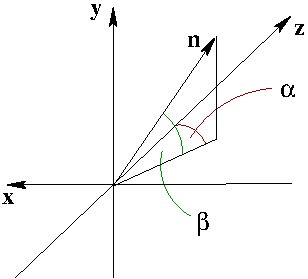
\includegraphics[origin=bl,height=60mm,angle=0]{./figures/rbendangle.pdf}
  %
  \caption{\label{rbendangle}
    Visualisation of angles used to rotate the face compared to the incoming beam. n is the normal of the face.
  }
  %
  \end{center}
%
\end{figure}

\subsection{\opalcycl mode}

This is a restricted feature: \noopalcycl .

\section{Quadrupoles}
\label{sec:quadrupole}
\index{QUADRUPOLE}
\begin{verbatim}
label:QUADRUPOLE,TYPE=string,APERTURE=real-vector,
          L=real,K1=real,K1S=real;
\end{verbatim}
A \texttt{QUADRUPOLE} has three real attributes:
\begin{description}
\item[L]
  \index{L}
  The quadrupole length (default: 0~m).
  A \secref{thin quadrupole}{thin} is defined by setting the length to zero. This is not valid for \opalt or \opalcycl.
\item[K1]
  \index{K1}
  The normal quadrupole component
  $K_1=\frac{1}{B \rho}\frac{\partial B_y}{\partial x}$.
  The default is $0 \mathrm{m}^{-2}$.
  The component is positive, if $B_y$ is positive on the positive $x$-axis.
  This implies horizontal focusing of positively charged particles which
  travel in positive $s$ direction.\\
  In \opalt $K_1=\frac{\partial B_y}{\partial x}$.
\item[K1S]
  \index{K1S}
  The skew quadrupole component
  $K_{1s}=\frac{1}{B \rho}\frac{\partial B_x}{\partial x}$.
  The default is $0 \mathrm{m}^{-2}$.
  The component is negative, if $B_x$ is positive on the positive $x$-axis.\\
In \opalt $K_{1s}=\frac{\partial B_x}{\partial x}$.
\end{description}
\noindent Example:
\begin{verbatim}
QF:QUADRUPOLE,L=1.5,K1=0.001;
\end{verbatim}
The reference system for a quadrupole is a 
\figref{Cartesian coordinate system}{straight}.

\subsection{\opalt mode}
\label{sec:quadrupole-t}
Using a quadrupole in OPAL-t mode, the following additional parameters are defined:
\begin{description}
\item[FMAPFN]
  \index{FMAPFN}
  Field maps in the {\em T7} format can be specified. This field map has to be of type \texttt{3DMagnetoStatic}
  or \texttt{1DMagnetoStaticEnge}. The latter type is used to calculate the Enge coefficients of the fringe fields.
  With help of this Enge coefficients the fringe field is constructed. Not yet implemented.
\item[ELEMEDGE]
  \index{ELEMEDGE}
  The edge of the field is specified absolute (floor space co-ordinates) in m.
  \end{description}
\noindent Example:
\begin{verbatim}
QP1: Quadrupole, L=1.20, ELEMEDGE=-0.5265, 
          FMAPFN="1T1.T7", K1=0.11;
\end{verbatim}

\subsection{\opalcycl mode}

This is a restricted feature:  \noopalcycl .

\section{Sextupoles}
\label{sec:sextupole}
\index{SEXTUPOLE}
\begin{verbatim}
label: SEXTUPOLE,TYPE=string,APERTURE=real-vector,
           L=real,K2=real,K2S=real;
\end{verbatim}
A \texttt{SEXTUPOLE} has three real attributes:
\begin{description}
\item[L]
  \index{L}
  The sextupole length (default: 0~m).
  A \secref{thin sextupole}{thin} is defined by setting the length to zero.
\item[K2]
  \index{K2}
  The normal sextupole component
  $K_2=\frac{1}{B \rho}\frac{\partial^2 B_y}{\partial x^2}$.
  The default is $0 \mathrm{m}^{-3}$.
  The component is positive, if $B_y$ is positive on the positive $x$-axis.
\item[K2S]
  \index{K2S}
  The skew sextupole component
  $K_{2s}=\frac{1}{B \rho}\frac{\partial^2 B_x}{\partial x^2}$.
  The default is $0 \mathrm{m}^{-3}$.
  The component is negative, if $B_x$ is positive on the positive $x$-axis.
\end{description}
\noindent Example:
\begin{verbatim}
S:SEXTUPOLE,L=0.4,K2=0.00134;
\end{verbatim}
The reference system for a sextupole is a 
\figref{Cartesian coordinate system}{straight}.
\subsection{\opalt mode}

\subsection{\opalcycl mode}

This is a restricted feature: \noopalt, \noopalcycl .

\section{Octupoles}
\label{sec:octupole}
\index{OCTUPOLE}
\begin{verbatim}
label:OCTUPOLE,TYPE=string,APERTURE=real-vector,
          L=real,K3=real,K3S=real;
\end{verbatim}
An \texttt{OCTUPOLE} has three real attributes:
\begin{description}
\item[L]
  \index{L}
  The octupole length (default: 0~m).
  A \secref{thin octupole}{thin} is defined by setting the length to zero.
\item[K3]
  \index{K3}
  The normal sextupole component
  $K_3=\frac{1}{B \rho}\frac{\partial^3 B_y}{\partial x^3}$.
  The default is $0 \mathrm{m}^{-4}$.
  The component is positive, if $B_y$ is positive on the positive $x$-axis.
\item[K3S]
  \index{K3S}
  The skew sextupole component
  $K_{3s}=\frac{1}{B \rho}\frac{\partial^3 B_x}{\partial x^3}$.
  The default is $0 \mathrm{m}^{-4}$.
  The component is negative, if $B_x$ is positive on the positive $x$-axis.
\end{description}
\noindent Example:
\begin{verbatim}
O3:OCTUPOLE,L=0.3,K3=0.543;
\end{verbatim}
The reference system for an octupole is a 
\figref{Cartesian coordinate system}{straight}.
\subsection{\opalt mode}

\subsection{\opalcycl mode}

This is a restricted feature: \noopalt, \noopalcycl .

\section{General Multipoles}
\label{sec:multipole}
\index{MULTIPOLE}
A \texttt{MULTIPOLE} is thin lens of arbitrary order, including a dipole:
\begin{verbatim}
label:MULTIPOLE,TYPE=string,APERTURE=real-vector,L=real,
      KNORMAL=real-vector,KSKEW=real-vector;
\end{verbatim}
\begin{description}
\item[L]
  \index{L}
  The multipole length (default: 0~m).
  A \secref{thin multipole}{thin} is defined by setting the length to zero.
\item[KN]
  \index{KN}
  A \secref{real vector}{anarray},
  containing the normal multipole coefficients.
  A component is positive, if $B_y$ is positive on the positive $x$-axis.
\item[KS]
  \index{KS}
  A \secref{real vector}{anarray},
  containing the skew multipole coefficients.
  A component is negative, if $B_x$ is positive on the positive $x$-axis.
\end{description}
The multipole coefficients are defined as
$K_{n} = \frac{1}{B \rho}\frac{\partial^n B_y}{\partial x^n}$.
(default: $0 \mathrm{m}^{-n}$).
The order $n$ is unlimited,
but all components up to the maximum must be given, even if zero.
The number of poles of each component is ($2 n + 2$).
The most important error components of fully symmetric quadrupoles are:
\texttt{KNORMAL[5]}, the 12-pole, and \texttt{KNORMAL[9]}, 
the twenty-pole.
Superposition of many multipole components is permitted.
The reference system for a multipole is a 
\figref{Cartesian coordinate system}{straight}.

\noindent Example:
\begin{verbatim}
M27:MULTIPOLE,L=1,KNORMAL[3]=0.0001,KSKEW[2]=0.0001;
\end{verbatim}
A multipole with no dipole component has no effect on the reference orbit,
i.e. the reference system at its exit is the same as at its entrance.
If it includes a dipole component,
it has the same effect on the reference orbit as a \texttt{SBEND}
with the same length and deflection angle \texttt{KNORMAL[0]*L}.
\subsection{\opalt mode}

\subsection{\opalcycl mode}

This is a restricted feature: \noopalt, \noopalcycl .

\section{Solenoids}
\label{sec:solenoid}
\index{SOLENOID}
\begin{verbatim}
label:SOLENOID,TYPE=string,APERTURE=real-vector,
          L=real,KS=real;
\end{verbatim}
A \texttt{SOLENOID} has two real attributes:
\begin{description}
\item[L]
  \index{L}
  The length of the solenoid (default: 0~m)
\item[KS]
  \index{KS}
  The solenoid strength $K_s$ (default: 0 rad/m).
  For positive \texttt{KS} and positive particle charge,
  the solenoid field points in the direction of increasing $s$.
\end{description}
\noindent Example:
\begin{verbatim}
SOLO:SOLENOID,L=2.,K=0.001;
\end{verbatim}
The reference system for a solenoid is a 
\figref{Cartesian coordinate system}{straight}.

\subsection{OPAL-t mode}
\label{sec:solenoid-t}
Using a solenoid in OPAL-t mode, the following additional parameters are defined:
\begin{description}
\item[FMAPFN]
  \index{FMAPFN}
  Field maps in the {\em T7} format can be specified.
\item[ELEMEDGE]
  \index{ELEMEDGE}
  The edge of the field is specified absolute (floor space co-ordinates) in m.
  \end{description}
\noindent Example:
\begin{verbatim}
SP1: Solenoid, L=1.20, ELEMEDGE=-0.5265, 
          FMAPFN="1T1.T7", KS=0.11;
\end{verbatim}

\subsection{\opalcycl mode}

This is a restricted feature: \noopalcycl .

\section{Cyclotron}
\label{sec:cyclotron}
\index{CYCLOTRON}
\begin{verbatim}
label:CYCLOTRON,TYPE=string, CYHARMON=int, 
          PHIINIT=real, PRINIT=real, RINIT=real, 
          SYMMETRY=real, RFFREQ=real, FMAPFN=string;
\end{verbatim}
A \texttt{CYCLOTRON} object includes the main characteristics of a cyclotron ,the magnetic field, 
 and also the initial condition of the injected reference particle, and it has currently the following attributes:
\begin{description}
\item[TYPE]
  \index{TYPE}
   The data format of field map, Currently three formats are implemented:
   CARBONCYCL, CYCIAE and default PSI format (Section \ref{sec:opalcycl:fildmap}).
\item[CYHARMON]
  \index{CYHARMON}
  The hamonic number of the cyclotron $h$. 
\item[RFFREQ]
  \index{RFFREQ}
  The first hamonic frequency of the RF system $f_{rf}$  (default: 0 MHz).
  The particle revolation frquency $f_{rev}$ =  $f_{rf}$ / $h$.
\item[FMAPFN]
  \index{FMAPFN}
  Filename for the magnetic field map. 
\item[SYMMETRY]
  \index{SYMMETRY}
  Defines symmetry characteristic of the B field map data stored in the file.  
\item[RINIT]
  \index{RINIT}
  The initial radius of reference particle (default: 0 mm)
\item[PHINIT]
  \index{PHINIT}
  The initial azimuth of reference particle (default: 0 deg)
\item[PRINIT]
  \index{PRINIT}
  Initial radial momenta of reference particle $P_r$=$\beta$$\gamma$ (doefaule : 0)
\end{description}
\noindent Example:
\begin{verbatim}
  ring: Cyclotron, TYPE="RING", CYHARMON=6, PHIINIT=0.0, 
           PRINIT=-0.000240, RINIT=2131.4 , SYMMETRY=8.0, 
           RFFREQ=50.650, FMAPFN="s03av.nar";
\end{verbatim}
The globe reference system for cyclotron is the Cartesian coordinate system.
Time is used as the  independent variable.
This is a restricted feature: \opalcycl .
\section{Orbit Correctors}
\label{sec:corrector}
\index{orbit corrector}
\index{KICKER}
\index{HKICKER}
\index{VKICKER}
Three types of closed orbit correctors are available:
\begin{description}
\item[HKICKER]
  \index{HKICKER}
  \label{sec:hkicker}
  A corrector for the horizontal plane,
\item[VKICKER]
  \index{VKICKER}
  \label{sec:vkicker}
  A corrector for the vertical plane,
\item[KICKER]
  \index{KICKER}
  \label{sec:kicker}
  A corrector for both planes.
\end{description}
\begin{verbatim}
label:HKICKER,TYPE=string,APERTURE=real-vector,
          L=real,KICK=real;
label:VKICKER,TYPE=string,APERTURE=real-vector,
          L=real,KICK=real;
label:KICKER, TYPE=string,APERTURE=real-vector,
          L=real,HKICK=real,VKICK=real;
\end{verbatim}
They have the following attributes:
\begin{description}
\item[L]
  \index{L}
  The length of the closed orbit corrector (default: 0~m).
\item[KICK]
  \index{KICK}
  The kick angle for either horizontal or vertical correctors.
  (default: 0~rad).
\item[HKICK]
  \index{HKICK}
  The horizontal kick angle for a corrector in both planes
  (default: 0~rad).
\item[VKICK]
  \index{VKICK}
  The vertical kick angle for a corrector in both planes
  (default: 0 rad).
\end{description}
A positive kick increases $p_{x}$ or $p_{y}$
respectively.

\noindent Examples:
\begin{verbatim}
HK1:HKICKER,KICK=0.001;
VK3:VKICKER,KICK=0.0005;
KHV:KICKER, HKICK=0.001,VKICK=0.0005;
\end{verbatim}
The first kicker is rotated about the longitudinal axis by 10 degrees.
The reference system for an orbit corrector is a 
\figref{Cartesian coordinate system}{straight}.

\subsection{\opalt mode}

\subsection{\opalcycl mode}

This is a restricted feature: \noopalt, \noopalcycl .

\section{RF Cavities}
\label{sec:cavity}
\index{RFCAVITY}
\index{cavity}
For an \texttt{RFCAVITY} the three modes have four real attributes in common:
\begin{verbatim}
label:RFCAVITY,APERTURE=real-vector,L=real,VOLT=real,LAG=real;
\end{verbatim}
\begin{description}
\item[L]
  \index{L}
  The length of the cavity (default: 0~m)
\item[VOLT]
  \index{VOLT}
  The peak RF voltage (default: 0~MV).
  The effect of the cavity is
  $\delta E=\mathtt{VOLT}\cdot\sin(2\pi(\mathtt{LAG}-\mathtt{HARMON}\cdot f_0 t))$.
\item[LAG]
  \index{LAG}
  The phase lag [$2\pi$] (default: 0).
\end{description}

\subsection{\opalmap mode}
The following attributes are supported only by the \opalmap mode
\begin{description}
\item[HARMON]
  \index{HARMON}
  The harmonic number $h$ (no default).
  Note that the RF frequency is computed from the harmonic number
  and the revolution frequency $f_0$.
  \textbf{The frequency attribute \texttt{FREQ} must no longer be used.}
\item[BETRF]
  \index{BETRF}
  RF coupling factor (default: 0).
\item[PG]
  \index{PG}
  The RF power per cavity (default: 0~mW).
\item[SHUNT]
  \index{SHUNT}
  The relative shunt impedance (default: $0 M\Omega/\mathrm{m}$).
\item[TFILL]
  \index{TFILL}
  The filling time of the cavity $T_\mathrm{fill}$
  (default: $0 \mu\mathrm{s}$).
\end{description}
Use of a cavity requires the particle momentum \texttt{P}
and the particle charge \texttt{CHARGE} to be set on the relevant 
optics command before any calculations is performed.

\noindent Example:
\begin{verbatim}
CAVITY:RFCAVITY,L=10.0,VOLT=150.0,LAG=0.0,HARMON=31320;
       STATIC,P=50.0,PARTICLE=ELECTRON;
\end{verbatim}
The reference system for a cavity is a 
\figref{Cartesian coordinate system}{straight}.

\subsection{\opalt mode}
\label{sec:cavity-t}
Using a RF Cavity in OPAL-t mode, the following additional parameters are defined:
\begin{description}
\item[FMAPFN]
  \index{FMAPFN}
  Field maps in the {\em T7} format can be specified.
\item[ELEMEDGE]
  \index{ELEMEDGE}
  The edge of the field is specified absolute (floor space co-ordinates) in m.
  \item[TYPE]
  \index{TYPE}
  Type specifies STANDING [default] or SINGLE GAP structures.   
  \item[FREQ]
  \index{FREQ}
  Defines the frequency of the RF Cavity in units of MHz. A warning is issued when the frequency of
  the cavity card does not correspond to the frequency defined in the   FMAPFN file. The  frequency of
  the cavity card overrides the  frequency defined in the  FMAPFN file.
  \end{description}
\noindent Example standing wave cavity which mimics a DC gun:
\begin{verbatim}
gun: RFCavity, L=0.018, VOLT=-131/(1.052*2.658), 
     FMAPFN="1T3.T7", ELEMEDGE=0.00, 
     TYPE="STANDING", FREQ=1.0e-6;
\end{verbatim}
\noindent Example of a two frequency standing wave cavity:
\begin{verbatim}
rf1: RFCavity, L=0.54, VOLT=19.961, LAG=193.0/360.0,
     FMAPFN="1T3.T7", ELEMEDGE=0.129, TYPE="STANDING", 
     FREQ=1498.956;
rf2: RFCavity, L=0.54, VOLT=6.250, LAG=136.0/360.0,
     FMAPFN="1T4.T7", ELEMEDGE=0.129, TYPE="STANDING", 
     FREQ=4497.536;
\end{verbatim}

\subsection{\opalcycl mode}
\label{sec:cavity-cycl}
Using a RF Cavity (standing wave) in \opalcycl mode, the following  parameters are defined:
\begin{description}
\item[FMAPFN]
  \index{FMAPFN}
  Defines name of file which stores normalized voltage amplitude curve of cavity gap in ASCII format.
  (See data format in Section\ref{sec:opalcycl:fildmap})
 \item[VOLT]
  \index{VOLT}
  Sets peak value of voltage amplitude curve in MV.
  \item[TYPE]
  \index{TYPE}
  Defines Cavity type, SINGLEGAP represents cyclotron type cavity.   
  \item[FREQ]
  \index{FREQ}
  Sets the frequency of the RF Cavity in units of MHz. 
  \item[RMIN]
  \index{RMIN}
  Sets the radius of the cavity inner edge in mm.
  \item[RMAX]
  \index{RMAX}
  Sets the radius of the cavity outer edge in mm.

  \item[ANGLE]
  \index{ANGLE}
  Sets the azimuthal position of the cavity in global frame in degree. 

  \item[PDIS]
  \index{PDIS}
  Set shift distance of cavity gap from center of cyclotron in mm. If its value is positive, 
  the shift direction is clockwise, namely, shift towards the smaller azimuthal angle.
  
  \item[GAPWIDTH]
  \index{GAPWIDTH}
  Set gap width of  cavity in mm.

  \item[PHI0]
  \index{PHI0}
  Set initial phase of cavity in degree.

\end{description}

\noindent Example of a RF cavity of cyclotron:
\begin{verbatim}
rf0: RFCavity, VOLT=0.25796, FMAPFN="Cav1.dat",
      TYPE="SINGLEGAP",FREQ=50.637, RMIN = 350.0,
      RMAX = 3350.0, ANGLE=35.0,   PDIS = 0.0,
      GAPWIDTH = 0.0, PHI0=phi01;
\end{verbatim}

Fig.\,\ref{figure_Cyclotron_cavity} shows the simplifed geometry of a cavity gap and its parameters.

\begin{figure}[hbt]
  \centering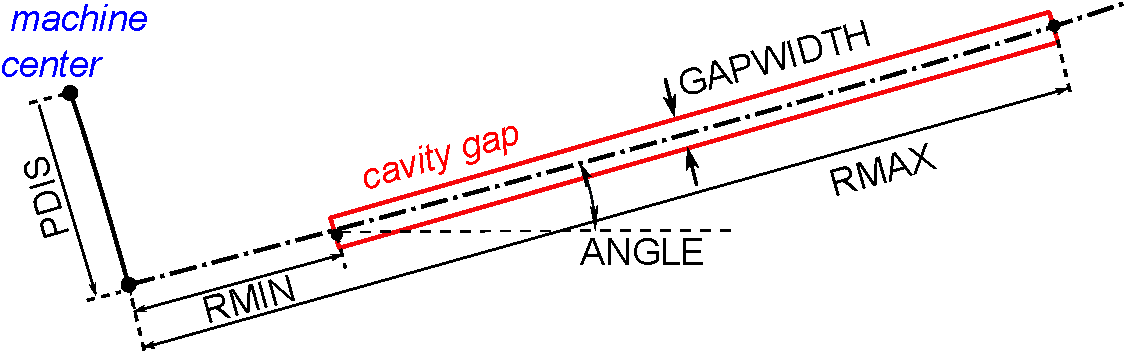
\includegraphics[scale=0.6]{./figures/cyclotron/Cavity.pdf}
  \caption{Schematic of the simplifed geometry of a cavity gap and parameters}
  \label{figure_Cyclotron_cavity}
\end{figure}


\section{Traveling Wave Structure}
\label{sec:travelingwave}
\index{TRAVELINGWAVE}

\begin{figure}[hbt]
  \centering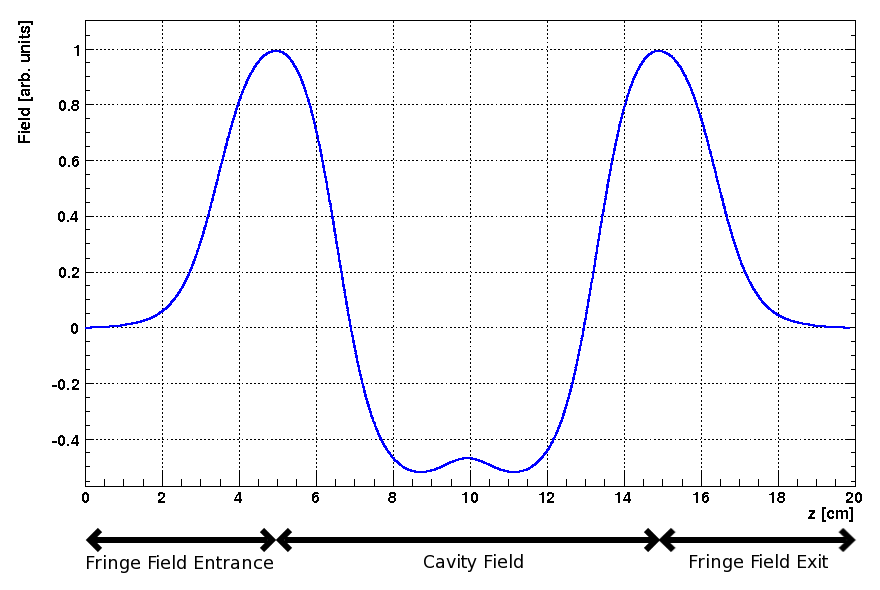
\includegraphics[scale=0.6]{./figures/traveling-wave-structure/FINSB-RAC-field.png}
  \caption{The field on axis for an S-band (2997.924~MHz) \texttt{TRAVELINGWAVE} structure.
    The field of a single cavity is shown between its entrance and exit fringe fields.
    The fringe fields extend one half wavelength ($\frac{\lambda}{2}$) to either side.}
  \label{figure_FINSB-RAC-field}
\end{figure}

\subsection{\opalt mode [only]}
An example of a 1D \texttt{TRAVELINGWAVE} structure field map is shown in Figure~\ref{figure_FINSB-RAC-field}.
This map is a standing wave solution generated by Superfish and shows the field on axis for a single accelerating cavity with
the fringe fields of the structure extending to either side. \opalt reads in this field map and constructs the total field of the
\texttt{TRAVELINGWAVE} structure in three parts: the entrance fringe field, the structure fields and the exit fringe field.

The fringe fields are treated as standing wave structures and are given by:
\begin{equation*}
  \begin{aligned}
    \vec{E_{entrance}}(\vec{r}, t) &= \vec{E_{from-map}}(\vec{r}) \cdot \text{VOLT} \cdot \cos \left[ 2\pi \left( \text{FREQ} \cdot t
        + \phi_{entrance} \right) \right] \\
    \vec{E_{exit}}(\vec{r}, t) &= \vec{E_{from-map}}(\vec{r}) \cdot \text{VOLT} \cdot \cos \left[ 2\pi \left( \text{FREQ} \cdot t
        + \phi_{exit} \right) \right]
  \end{aligned}
\end{equation*}
where VOLT and FREQ are the field magnitude and frequency attributes (see below). 
$ \phi_{entrance}= \text{LAG}$, the phase attribute of the element (see below). $ \phi_{exit} $ is dependent upon both LAG and the NUMCELLS
attribute (see below) and is calculated internally by \opalt.

The field of the main accelerating structure is reconstructed from the center section of the standing wave solution shown in
Figure~\ref{figure_FINSB-RAC-field} using

\begin{equation*}
  \begin{split}
    \vec{E} ( \vec{r},t ) &= \frac{\text{VOLT}}{\sin (2 \pi \cdot \text{MODE})} \\
    &\phantom{=}
    \times \Biggl\{ \vec{E_{from-map}} (x,y,z) \cdot \cos \biggl[ 2 \pi \Bigl( \text{FREQ} \cdot t + \text{LAG} \\
    &\phantom{= \times \Biggl\{ \vec{E_{from-map}} (x,y,z) \cdot \cos \biggl[ 2 \pi \Bigl(}
    + \frac{\pi}{2} \cdot \text{MODE} \Bigr) \biggr] \\
    &\phantom{= \times \Biggl\{}
    + \vec{E_{from-map}}(x,y,z+d) \cdot \cos \biggl[ 2 \pi \Bigl( \text{FREQ} \cdot t + \text{LAG} \\
    &\phantom{= \times \Biggl\{ + \vec{E_{from-map}} (x,y,z+d) \cdot \cos \biggl[ 2 \pi \Bigl(}
    + \frac{3 \pi}{2} \cdot \text{MODE} \Bigr) \biggr] \Biggr\}
  \end{split}
\end{equation*}
where d is the cell length and is defined as $\text{d} = \lambda \cdot \text{MODE} $. MODE is an attribute of the element (see below).
When calculating the field from the map ($\vec{E_{from-map}}(x,y,z)$), the longitudintal position is referenced to the start of the cavity fields
at $\frac{\lambda}{2}$ (In this case starting at $z = 5.0 \text{ cm}$). If the longitudinal position advances past the end of the cavity map
($\frac{3\lambda}{2} = 15.0 \text{ cm}$ in this example), an integral number of cavity wavelenths is subtracted from the position until it is back
within the map's longitudinal range.

A \texttt{TRAVELINGWAVE} structure has seven real attributes, one integer attribute, one string attribute and one boolean attribute:
\begin{verbatim}
label:TRAVELINGWAVE, APERTURE=real-vector, L=real,
      VOLT=real, LAG=real, FMAPFN=string,
      ELEMEDGE=real, FREQ=real, NUMCELLS=integer,
      MODE=real;
\end{verbatim}

\begin{description}
\item[L]
  \index{L}
  The length of the cavity (default: 0~m).
\item[VOLT]
  \index{VOLT}
  The peak RF voltage (default: 0~MV).
  The effect of the cavity is
  $\delta E=\mathtt{VOLT}\cdot\sin(2\pi(\mathtt{LAG}- \mathtt{FREQ}\cdot t))$.
\item[LAG]
  \index{LAG}
  The phase lag [$2\pi$] (default: 0).
\item[FMAPFN]
  \index{FMAPFN}
  Field maps in the {\em T7} format can be specified.
\item[ELEMEDGE]
  \index{ELEMEDGE}
  The edge of the field is specified absolute (floor space co-ordinates) in m. This is the position of the front edge
  of the first \texttt{TRAVELINGWAVE} cavity. (In the simulation the actual field will extend $\frac{1}{2}$ wavelength
  in front of this position.)
\item[FREQ]
  \index{FREQ}
  Defines the frequency of the traveling wave structure in units of MHz. A warning is issued when the frequency of
  the cavity card does not correspond to the frequency defined in the  FMAPFN file. The frequency defined in the FMAPFN
  file overrides the frequency defined on the cavity card. 
\item[NUMCELLS]
  \index{NUMCELLS}
  Defines the number of cells in the tank. (The cell count should not include the entry and exit half cell fringe fields.)
\item[MODE]
  \index{MODE}
Defines the mode in units of $2\pi$, for example $\frac{1}{3}$ stands for a $\frac{2 \pi}{3}$ structure.
\item[FAST]
  \index{FAST}
If FAST is true and the provided fieldmap is in 1D then a 2D fieldmap is constructed from the 1D on-axis field, see section~\ref{sec:fieldmaps}. To track the particles the field values are interpolated from this map instead of using an FFT based algorithm for each particle and each step. (default: FALSE)
\end{description}

\noindent Use of a traveling wave requires the particle momentum \texttt{P}
and the particle charge \texttt{CHARGE} to be set on the relevant 
optics command before any calculations are performed.
\\\\
\noindent Example of a L-Band travelling wave structure:
\begin{verbatim}
lrf0: TravelingWave, L=0.0253, VOLT=14.750,
      NUMCELLS=40, ELEMEDGE=2.73066,
      FMAPFN="INLB-02-RAC.Ez", MODE=1/3,
      FREQ=1498.956, LAG=248.0/360.0;
\end{verbatim}

\section{Electrostatic Separators}
\label{sec:separator}
\index{ELSEPARATOR}
\index{separator}
An \texttt{ELSEPARATOR} (electrostatic separator) has three real
attributes:
\begin{verbatim}
label:ELSEPARATOR,TYPE=string,APERTURE=real-vector,
L=real,EX=real,EY=real;
\end{verbatim}
\begin{description}
\item[L]
  \index{L}
  The length of the separator (default: 0~m).
\item[EX]
  \index{EX}
  The horizontal electric field strength (default: 0~MV/m).
  A positive field increases $p_x$ for positive particles.
\item[EY]
  \index{EY}
  The vertical electric field strength (default: 0~MV/m).
  A positive field increases $p_y$ for positive particles.
\end{description}
A \texttt{ELSEPARATOR} requires the particle momentum \texttt{P} 
and its charge \texttt{CHARGE} to be set in the relevant
\secref{\texttt{BEAM} command}{beam} before any calculations are performed.

\noindent Example:
\begin{verbatim}
BEAM,PARTICLE=POSITRON,PC=46.0;
SEP:ELSEPARATOR,L=5.0,E=0.5;
\end{verbatim}
The reference system for a separator is a 
\figref{Cartesian coordinate system}{straight}.
\subsection{\opalt mode}

\subsection{\opalcycl mode}

This is a restricted feature: \noopalt, \noopalcycl .

\section{Beam Position Monitors}
\label{sec:monitors}
\index{MONITOR}
\index{HMONITOR}
\index{VMONITOR}
A beam monitor acts on the beam like a drift space.
In addition it records the beam position for closed orbit
corrections. 
Four different types of beam position monitors are recognised:
\begin{description}
\item[HMONITOR]
  \label{sec:hmonitor}
  Monitor for the horizontal beam position,
\item[VMONITOR]
  \label{sec:vmonitor}
  Monitor for the vertical beam position,
\item[MONITOR]
  \label{sec:monitor}
  Monitor for both horizontal and vertical beam position.
\item[INSTRUMENT]
  \label{sec:instrument}
  A place holder for any other type of beam instrumentation.
  Optically it behaves like a drift space;
  it returns \textbf{no beam observation}.
  It represents a class of elements
  which is completely independent from drifts and monitors.
\end{description}
\begin{verbatim}
label:HMONITOR,  TYPE=string,APERTURE=real-vecto,L=real;
label:VMONITOR,  TYPE=string,APERTURE=real-vecto,L=real;
label:MONITOR,   TYPE=string,APERTURE=real-vecto,L=real;
label:INSTRUMENT,TYPE=string,APERTURE=real-vector,L=real;
\end{verbatim}
A beam position monitor has one real attribute:
\begin{description}
\item[L]
  \index{L}
  The length of the monitor (default: 0~m). 
  If the length is different from zero,
  the beam position is recorded in the centre of the monitor
  (except for the \texttt{INSTRUMENT} element).
\end{description}
\noindent Examples:
\begin{verbatim}
MH:HMONITOR,L=1;
MV:VMONITOR;
\end{verbatim}
The reference system for a monitor is a 
\figref{Cartesian coordinate system}{straight}.
\subsection{\opalt mode}
Not supported are \texttt{HMONITOR}, \texttt{VMONITOR} and \texttt{INSTRUMENT}. A \texttt{MONITOR} detects all particles passing it and writes the position, the momentum and the time when they hit it into an H5Part file. Furthermore the exact position of the monitor is stored. It has always a length of $1\; cm$ consisting of $0.5\;cm$ drift, the monitor of zero length and another $0.5\;cm$ drift. This is to prevent \opalt from missing any particle. The positions of the particles on the monitor are interpolated from the current position and momentum one step before they would passe the monitor.
\begin{description}
\item[OUTFN]
  \index{OUTFN}
  The filename into which the monitor should write the collected data. The file is an H5Part file.
\item[ELEMEDGE]
  \index{ELEMEDGE}
  The position of the monitor is specified absolute (floor space co-ordinates) in m. This is the position at which the data is collected.
\end{description}

\subsection{\opalcycl mode}

This is a restricted feature:  \noopalcycl .

%\section{Gun}
%\label{sec:gun}
%\index{gun}
%The gun uses the defined distribution (Section \ref{sec:distribution}) and emits particles for a given duration (eventually defined
%by the laser duration).  The temperature is defined by the parameters on the distribution command.

%\begin{verbatim}
%g1:GUN, TYPE=string, TEMISSION=real, L=real, EMISSIONSLICES=real;
%\end{verbatim}
%The gun has beside the standard attribute TYPE,  four more attributes:
%\begin{description}
%\item[L]
%  \index{L}
%  The gun length (default: 0~m).
%\item[TEMISSION]
%  \index{TEMISSION}
%  The time-span  at which emission occurs (default: 0~sec).
%\item[EMISSIONSLICES]
%  \index{EMISSIONSLICES}
%  How many emission slices we consider (default: 0).
%\end{description}

%\noindent Example:
%\begin{verbatim}
%G1:GUN, L=6.0E-3, TEMISSION= 36E-12, EMISSIONSLICES=360;
%\end{verbatim}
%The reference system for a gun is a 
%\figref{Cartesian coordinate system}{straight}.

\section{Collimators}
\label{sec:collimators}
\index{collimator}
\index{ECOLLIMATOR}
\index{RCOLLIMATOR}
Two types of collimators are defined:
\begin{description}
\item[ECOLLIMATOR]
  \label{sec:ecollimator}
  Elliptic aperture,
\item[RCOLLIMATOR]
  \label{sec:rcollimator}
  Rectangular aperture.
\end{description}
\begin{verbatim}
label:ECOLLIMATOR,TYPE=string,APERTURE=real-vector,L=real,
      XSIZE=real,YSIZE=real;
label:RCOLLIMATOR,TYPE=string,APERTURE=real-vector,L=real,
      XSIZE=real,YSIZE=real;
\end{verbatim}
Either type has three real attributes:
\begin{description}
\item[L]
  \index{L}
  The collimator length (default: 0~m).
\item[XSIZE]
  \index{XSIZE}
  The horizontal half-aperture (default: unlimited).
\item[YSIZE]
  \index{YSIZE}
  The vertical half-aperture (default: unlimited).
\end{description}
For elliptic apertures,
\texttt{XSIZE} and \texttt{YSIZE} denote the half-axes respectively,
for rectangular apertures they denote the half-width of the rectangle.
Optically a collimator behaves like a drift space, but during tracking,
it also introduces an aperture limit.
The aperture is checked at the entrance.
If the length is not zero, the aperture is also checked at the exit.

\noindent Example:
\begin{verbatim}
COLLIM:ECOLLIMATOR,L=0.5,XSIZE=0.01,YSIZE=0.005;
\end{verbatim}
The reference system for a collimator is a 
\figref{Cartesian coordinate system}{straight}.


\subsection{\opalt mode}
Not supported at the moment is the \texttt{RCOLLIMATOR}. A \texttt{ECOLLIMATOR} detects all particles which are outside the aperture defined by
\texttt{XSIZE} and \texttt{YSIZE}. The lost particles are saved  into an H5Part file defined by \texttt{OUTFN}.  The \texttt{ELEMEDGE} defines the
location of the collimator and \texttt{L} the length.
\begin{description}
\item[OUTFN]
  \index{OUTFN}
  The filename into which the monitor should write the collected data. The file is an H5Part file.
\item[ELEMEDGE]
  \index{ELEMEDGE}
  The position of the monitor is specified absolute (floor space co-ordinates) in m. This is the position at which the data is collected.
\end{description}

\noindent Example:
\begin{verbatim}
Col:ECOLLIMATOR, L=1.0E-3, ELEMEDGE=3.0E-3, XSIZE=5.0E-4, 
       YSIZE=5.0E-4, OUTFN="Coll.h5";
\end{verbatim}


\subsection{\opalcycl mode}

This is a restricted feature: \noopalcycl .

\section{Coordinate Transformations}
\label{sec:rotation}

\subsection{Rotations About the Vertical Axis}
\label{sec:yrot}
\index{rotation}
\index{coordinate!change}
\index{YROT}
\begin{verbatim}
label:YROT,TYPE=string,APERTURE=real-vector,ANGLE=real;
\end{verbatim}
The element \texttt{YROT} rotates reference system 
\figref{about the vertical ($y$) axis}{yrot}.
\texttt{YROT} has no effect on the beam,
but it causes the beam to be referred to the new coordinate system
\[\begin{array}{lcl}
  x_2&=&x_1\cos\theta-s_1\sin\theta, \\
  y_2&=&x_1\sin\theta+s_1\cos\theta,
\end{array}\]
It has one real attribute:
\begin{description}
\item[ANGLE]
  \index{ANGLE}
  The rotation angle theta (default: 0 rad).
  It must be a \textbf{small} angle,
  i.e. an angle comparable to the transverse angles of the orbit.
\end{description}
A positive angle means that the new reference system is rotated
clockwise about the local $y$-axis with respect to the old system.

\noindent Example:
\begin{verbatim}
KINK:YROT,ANGLE=0.0001;
\end{verbatim}

\subsection{Rotations Around the Longitudinal Axis}
\label{sec:srot}
\index{rotation}
\index{coordinate!change}
\index{SROT}
\begin{verbatim}
label:SROT,TYPE=string,APERTURE=real-vector,ANGLE=real;
\end{verbatim}
The element \texttt{SROT} rotates the reference system
\figref{about the longitudinal ($s$) axis}{srot}.
\texttt{SROT} has no effect on the beam,
but it causes the beam to be referred to the new coordinate system
\[\begin{array}{lcl}
  x_2&=&x_1\cos\psi-y_1\sin\psi, \\
  y_2&=&x_1\sin\psi+y_1\cos\psi,
\end{array}\]
It has one real attribute:
\begin{description}
\item[ANGLE]
  \index{ANGLE}
  The rotation angle psi (default: 0~rad)
\end{description}
A positive angle means that the new reference system is rotated clockwise
about the $s$-axis with respect to the old system.

\noindent Example:
\begin{verbatim}
ROLL1:SROT,ANGLE=PI/2.;
ROLL2:SROT,ANGLE=-PI/2.;
HBEND:SBEND,L=6.0,ANGLE=0.01;
VBEND:LINE=(ROLL1,HBEND,ROLL2);
\end{verbatim}
The above is a way to represent a bend down in the vertical plane,
it could be defined more simply by
\begin{verbatim}
VBEND:SBEND,L=6.0,K0S=-0.01/6.0;
\end{verbatim}

\subsection{General Change of Reference}
\label{sec:patch}
\index{reference!change}
\index{coordinate!change}
\index{PATCH}
\begin{verbatim}
label:PATCH,TYPE=string,APERTURE=real-vector,
	DX=real,DY=real,DZ=real,DTHETA=real,
	DPHI=real,DPSI=real;
\end{verbatim}
The element \texttt{PATCH} applies a general change to the reference system. 
\texttt{PATCH} has no effect on the beam,
but it causes the beam to be referred to the new coordinate system.
It has six real attributes:
\begin{description}
\item[DX]
  \index{DX}
  The displacement in $x$-direction of the new system with respect to the old
  one. 
\item[DY]
  \index{DY}
  The displacement in $y$-direction of the new system with respect to the old
  one. 
\item[DS]
  \index{DS}
  The displacement in $s$-direction of the new system with respect to the old
  one. 
\item[VX]
  \index{VX}
  The rotation around the $x$-axis of the new system with respect to the old
  one. 
\item[VY]
  \index{VY}
  The rotation around the $y$-axis of the new system with respect to the old
  one. 
\item[VZ]
  \index{VZ}
  The rotation around the $s$-axis of the new system with respect to the old
  one. 
\end{description}

\noindent As an example consider a simplified model of the
\figref{separation of the two beams}{patch} near the interaction region of
LHC:
\begin{verbatim}
ALPHA=...;    // The bend angle in the separator magnets.
DISTANCE=...; // The longitudinal distance between
			// the separator magnets.
D1:HKICKER,L=0,KICK=ALPHA;
D2:HKICKER,L=0,KICK=-ALPHA;
DIST:DRIFT,L=DISTANCE;
PATCH1:PATCH,DX=DISTANCE*TAN(ALPHA);
PATCH2:PATCH,DX=-DISTANCE*TAN(ALPHA);
SHARED SEPARATION:LINE=(D1,DIST,D2);
RING1:SEQUENCE,...; // beam goes clockwise.
...
SEPARATION;
PATCH1;             // change reference to 
...
ENDSEQUENCE;
RING2:SEQUENCE,...; // beam goes anticlockwise.
...
SEPARATION;
PATCH2;
...
ENDSEQUENCE;
\end{verbatim}
The direction of travel of each beam determines the signs of the deflections, 
the patches change the reference.
Note that the common reference between the two separator magnets allows a
correct handling of long-distance beam-beam interactions in that area.
\begin{figure}[ht]
  \begin{center}
    \begin{picture}(400,90)
      \thinlines
      \drawline(0,40)(100,40)
      \drawline(100,40)(200,60)(300,60)
      \put(240,65){\vector(1,0){20}}
      \put(305,60){\makebox(0,0)[l]{reference beam 1}}
      \dashline[30]{8}(100,40)(200,40)
      \put(205,40){\makebox(0,0)[l]{common reference}}
      \drawline(100,40)(200,20)(300,20)
      \put(260,15){\vector(-1,0){20}}
      \put(305,20){\makebox(0,0)[l]{reference beam 2}}

      \drawline(100,10)(100,70)
      \put(100,75){\makebox(0,0)[b]{\texttt{D1}}}
      \drawline(200,10)(200,70)
      \put(200,75){\makebox(0,0)[b]{\texttt{D2}+patches}}
    \end{picture}
    \caption{Separation of two beams}
    \label{fig:patch}
  \end{center}
\end{figure}

This is a restricted feature: \noopalt, \noopalcycl .
%
%\section{Beam-Beam Interactions}
%\label{sec:beambeam}
%\index{BEAMBEAM}
%\index{interaction!beam-beam}
%The command \texttt{BEAMBEAM} may be inserted in a beam line
%to simulate a beam-beam interaction point:
%\begin{verbatim}
%label:BEAMBEAM,TYPE=string,APERTURE=real-vector,
%      SIGX=real,SIGY=real,XMA=real,YMA=real,CHARGE=real;
%\end{verbatim}
%The code for this element has been contributed by J.M. Veuillen (1987),
%and has been adapted to C++ in 1997.
%It has six real attributes:
%\begin{description}
%\item[SIGX]
%  \index{SIGX}
%  The horizontal extent (standard deviation) of the opposite beam
%  (default: 0~m).
%\item[SIGY]
%  \index{SIGY}
%  The vertical extent (standard deviation) of the opposite beam
%  (default: 0~m).
%\item[XMA]
%  \index{XMA}
%  The horizontal displacement of the opposite beam with respect to
%  the ideal orbit (default: 0~m).
%\item[YMA]
%  \index{YMA}
%  The vertical displacement of the opposite beam with respect to
%  the ideal orbit (default: 0~m).
%\item[CHARGE]
%  \index{CHARGE}
%  The charge of particles in the opposite beam in proton charges
%  (default: 0).
%\item[NPART]
%  \index{NPART}
%  The number of particles in the opposite beam.
%  (default: 0).
%\end{description}
%A beam-beam element requires the particle momentum \texttt{P}
%and its charge \texttt{CHARGE} to be defined on the relevant optics command
%before any calculations are performed.

%\noindent Example:
%\begin{verbatim}
%BEAM,MOMENTUM=46.0,MASS=PMASS,CHARGE=1.0;
%BB:BEAMBEAM,SIGX=1.E-3,SIGY=5.E-4,CHARGE=1.0,NPART=1.0E12;
%\end{verbatim}

%A three-dimensional representation of a beam-beam interaction is
%available with the command
%\index{BEAMINT}
%\index{interaction!beam-beam}
%\begin{verbatim}
%label:BEAMINT,TYPE=string,APERTURE=real-vector,
%      PHI=real,NSLI=integer,FAST=bool,XIYN=real,DX=real,DY=real,DZ=real,
%      BETXS=real,BETYS=real,ALFXS=real,ALFYS=real,
%      DXS=real,DPXS=real,DYS=real,DPYS=real,
%      EXS=real,EYS=real,SIGTS=real,SIGES=real;
%\end{verbatim}
%Its parameters are:
%\begin{description}
%\item[PHI]
%  \index{PHI}
%  Horizontal crossing angle.
%\item[NSLI]
%  \index{NSLI}
%  Number of slices to be taken in strong beam.
%\item[FAST]
%  \index{FAST}
%  If true, use tables for computing the error function.
%\item[XIYN]
%  \index{XIYN}
%  Beam-beam parameter.
%\item[DX]
%  \index{DX}
%  Horizontal displacement of the interaction point in [m].
%\item[DY]
%  \index{DY}
%  Vertical displacement of the interaction point in [m].
%\item[DZ]
%  \index{DZ}
%  Longitudinal displacement of the interaction point in [m].
%\end{description}
%The following parameters describe the strong beam:
%\begin{description}
%\item[BETXS]
%  \index{BETXS}
%  Horizontal $\beta*$ in [m].
%\item[BETYS]
%  \index{BETYS}
%  Vertical $\beta*$ in [m].
%\item[ALFXS]
%  \index{ALFXS}
%  Horizontal $\alpha*$* in [1].
%\item[ALFYS]
%  \index{ALFYS}
%  Vertical $\alpha*$ in [1].
%\item[DXS]
%  \index{DXS}
%  Horizontal dispersion in [m].
%\item[DPXS]
%  \index{DPXS}
%  Horizontal dispersion slope in [m].
%\item[DYS]
%  \index{DYS}
%  Vertical dispersion in [m].
%\item[DPYS]
%  \index{DPYS}
%  Vertical dispersion slope in [m].
%\item[EXS]
%  \index{EXS}
%  Horizontal emittance in [m rad].
%\item[EYS]
%  \index{EYS}
%  Vertical emittance in [m rad].
%\item[SIGTS]
%  \index{SIGTS}
%  Bunch length in [m].
%\item[SIGES]
%  \index{SIGES}
%  Energy spread in [1].
%\end{description}  

\section{Editing Element Definitions}
\label{sec:elm-edit}
\index{element!editing}
\index{edit!element}
An element definition can be changed in two ways:
\begin{description}
\item[Entering a new definition]
  The element definition will be replaced.
  A beam element, \secref{\texttt{LINE}}{line}, 
  or \secref{\texttt{SEQUENCE}}{sequence}
  can be replaced by another beam element, beam line, or sequence;
  if the replaced item occurs in another beam line or sequence,
  all references in that line or sequence are replaced.
\item[Entering the element name together with new attributes]
  The element will be updated in place,
  and the new attribute values will replace the old ones.
  When the type of the element should not change,
  replacement of an attribute is the more efficient way.
\end{description}
Element definitions can be changed freely.
The changes do not affect already defined objects which belong to
its \secref{class}{elm-class}.
This example shows two ways to change the strength of a quadrupole:
\begin{verbatim}
QF:QUADRUPOLE,L=1,K1=0.01; // Original definition of QF
QF:QUADRUPOLE,L=1,K1=0.02; // Replace whole definition of QF
QF,K1=0.02;                // Replace value of K1
\end{verbatim}
\subsection{\opalt mode}

\subsection{\opalcycl mode}

This is a restricted feature: \noopalt, \noopalcycl .

\section{Wake Functions}
Three types of wake functions are implemented so far: transverse and longitudinal geometric wakes and the CSR wake. The general input format is
\begin{verbatim}
label:WAKE, TYPE=string,NBIN=real,CONST_LENGTH=bool,
      CONDUCT=string,Z0=real,FORM=string,RADIUS=real,
      SIGMA=real,TAU=real,FILTERS=string-array
\end{verbatim}
CONST\_LENGTH, CONDUCT, Z0, FORM, RADIUS, SIGMA and TAU are only used in the geometric wakes.
\begin{description}
\item[TYPE]
  \index{TYPE}
  The type of wake function; either TRANSV-SHORT-RANGE, LONG-SHORT-RANGE or 1D-CSR.
\item[NBIN]
  \index{NBIN}
  Not implemented yet; Number of bins to be used for line density if different from space charge solver grid.
\item[CONST\_LENGTH]
  \index{CONST\_LENGTH}
  
\item[CONDUCT]
  \index{CONDUCT}

\item[Z0]
  \index{Z0}

\item[FORM]
  \index{FORM}

\item[RADIUS]
  \index{RADIUS}

\item[SIGMA]
  \index{SIGMA}

\item[TAU]
  \index{TAU}

\item[FILTERS]
  \index{FILTERS}
  Array of names of filters to be applied onto the longitudinal histogram of the bunch to get rid of the noise and to calculate derivatives. All the filters/smoothers are applied to the line density in the order they appear in the array. The last filter is also used for calculating the derivatives. The actual filters have to be defined elsewhere.
\end{description}

\section{Filters}
Filters can be defined which then are applied to the line density of the bunch. The following smoothing filters are implemented: Savitzky-Golay, Stencil, FixedFFTLowPass, RelativFFTLowPass. The input format for them is
\begin{verbatim}
label:FILTER, TYPE=string, NFREQ=real, THRESHOLD=real, 
      NPOINTS=real, NLEFT=real, NRIGHT=real, 
      POLYORDER=real
\end{verbatim}
\begin{description}
\item[TYPE]
  \index{TYPE}
  The type of filter: Savitzky-Golay, Stencil, FixedFFTLowPass, RelativFFTLowPass
\item[NFREQ]
  \index{NFREQ}
  Only used in FixedFFTLowPass: the number of frequencies to keep
\item[THRESHOLD]
  \index{THRESHOLD}
  Only used in RelativeFFTLowPass: the minimal strength of frequency compared to the stronges to consider.
\item[NPOINTS]
  \index{NPOINTS}
  Only used in Savitzky-Golay: width of moving window in number of points
\item[NLEFT]
  \index{NLEFT}
  Only used in Savitzky-Golay: number of points to the left
\item[NRIGHT]
  \index{NRIGHT}
  Only used in Savitzky-Golay: number of points to the right
\item[POLYORDER]
  \index{POLYORDER}
  Only used in Savitzky-Golay: polynomial order to be used in least square approximation
\end{description}
The Savitzky-Golay filter and the ones based on the FFT routine provide a derivative on a natural way. For the Stencil filter a second order stencil is used to calculate the derivative.

An implementation of the Savitzky-Golay filter can be found in the Numerical Recipes. The Stencil filter uses the following two stencil consecutively to smooth the line density:
$$f_i = \frac{7\cdot f_{i-4} + 24\cdot f_{i-2} + 34\cdot f_{i} + 24\cdot f_{i+2} + 7\cdot f_{i+4}}{96}$$
and
$$f_i = \frac{7\cdot f_{i-2} + 24\cdot f_{i-1} + 34\cdot f_{i} + 24\cdot f_{i+1} + 7\cdot f_{i+2}}{96}.$$
For the derivative a standard second order stencil is used:
$$f^{\prime}_i = \frac{f_{i-2} - 8\cdot f_{i-1} + 8\cdot f_{i+1} - f_{i+2}}{h}$$
This filter was designed by Ilya Pogorelov for the ImpactT implementation of the CSR 1D model.

The FFT based smoothers calculate the Fourier coefficients of the line density. Then they set all coefficients corresponding to frequencies above a certain threshold to zero. Finally the back-transformation is calculate using this coefficients. The two filters differ in the way they identify coefficients which should be set to zero. FixedFFTLowPass uses the n lowest frequencies whereas RelativeFFTLowPass searches for the coefficient which has the biggest absolut value. All coefficients which, compared to this value, are below a threshold (measure in percents) are set to zero. For the derivative the coefficients are multiplied with the following function (this is equivalent to a convolution): 
$$g_{i} = 
\begin{cases}
i \frac{2\pi \imath}{N\cdot L} & i < N/2 \\
-i \frac{2\pi \imath}{N\cdot L} & i > N/2
\end{cases}$$
where $N$ is the total number of coefficients/sampling points and L is the length of the bunch.
\index{element|)}
